\documentclass[a4paper, 12pt]{report}
\usepackage[utf8]{inputenc}
\usepackage[boxed,linesnumbered]{algorithm2e}
\usepackage[bookmarks, breaklinks, colorlinks]{hyperref}

\hypersetup{
	citecolor=black,
	linkcolor=black,
	filecolor=black,
	urlcolor=black
}

\usepackage{graphicx}
\usepackage{pdfpages}
\usepackage{tocbibind}
\usepackage{longtable}
\usepackage{array}

\def\chapterautorefname{Chapter}


\title{
	\begin{figure}[h]
		\centering
		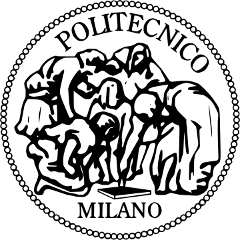
\includegraphics{../common_resources/logo_polimi.png}
	\end{figure}
	\vspace{30px}
	Software Engineering 2 Project: PowerEnJoy \\ \vspace{1em}
	\textbf{I}ntegration \textbf{T}est \textbf{P}lan \textbf{D}ocument
}
	

\author{Marco Ieni, Francesco Lamonaca, Marco Miglionico\\Politecnico di Milano, A.A. 2016/2017}
\date{\today\\v1.0}

\begin{document}
\maketitle
\tableofcontents
% \listoffigures
% \listoftables

\chapter{Introduction}
\label{ch:introduction}
\section{Revision History}
\section{Purpose and Scope}
This document is the Integration Test Plan Document (ITPD) for the PowerEnJoy
software. Its purpose is to determine how to accomplish the
integration test of the software, which tools need to be used and which approach
will be followed.
Integration testing is fundamental activity to guarantee that all the different components of PowerEnjoy interoperate consistently with the requirements they are supposed to fulfil and without unexpected behaviours.
In the following sections we are going to provide:
\begin{itemize}
\item A list of the components and their subcomponents involved in the integration activity that will be tested;
\item The criteria that must be met by the project status before integration testing of the outlined elements may begin;
\item A description of the integration testing approach and the reasoning behind it;
\item The sequence in which the different components will be integrated;
\item A description of the planned testing activities for each integration step, including their input data and the expected output;
\item Some performance measures that should be performed on the components to check that they are fulfilling the requirements;
\item A list of all the tools that will have to be employed during the testing activities, together with a description of the operational environment in which the tests will be executed.
\end{itemize} 

\section{Definitions, acronyms, abbreviations}
\begin{description}
    \item[JPA:] The Java Persistence API (JPA) is a Java application programming interface specification that describes the management of relational data.
    \item[RASD:] Requirements Analysis and Specification Document.
\end{description}

\section{Reference Documents}
This document refers to the project rules of the Software Engineering 2
project, to the template for the Design Document contained into it and to Requirement Analysis and Specification Document (the previous delivered document)


\chapter{Integration Strategy}
\label{ch:integration_strategy}
\section{Entry Criteria}
% Specify the criteria that must be met before integration testing of specific elements may begin (e.g., functions must have been unit tested).
\section{Elements to be Integrated}
In the following paragraph we are going to provide a list of all the components that need to be integrated together.

The integration process of our software is performed on two levels.
\begin{enumerate}
\item \textbf{Low Level:} integration of the different subcomponents (classes, Java Beans) inside the
same subsystem;
\item \textbf{High Level:} integration of different subsystems.
\end{enumerate}

The first step needs to be performed only for the components which contains
the pieces of software that we are going to develop, namely the business
tier, the mobile application in the client tier.
In particular the main subcomponents  that we will integrate are:
\begin{itemize}
\item \textbf{User Manager};
\item \textbf{Email Sender};
\item \textbf{Operator Safe Area Manager};
\item \textbf{User Safe Area Manager};
\item \textbf{Ride Manager};
\item \textbf{Car Manager};
\item \textbf{Fee Manager};
\item \textbf{Payment Manager}
\end{itemize}


The second step need to be performed on the three major high-level components that we outlined in the Design Document,that correspond to the tiers of the system, which – from now on – will
be referred to as subsystems:
\begin{itemize}
\item \textbf{Client tier:} The client tier consists of our mobile application,the operator terminal and the on-board tablet.
\item\textbf{Business tier:} This subsystem implements all the application logic and
communicates with the front-ends.
\item \textbf{Database tier:} This is the DBMS,it is not part of the software to be developed,
but has to be integrated.
\end{itemize}




\section{Integration Testing Strategy}
The integration strategy that we are going to implement is the bottom-up approach. This choice
comes natural since we assume we already have the unit tests for the smallest
components, so we can proceed from the bottom.In this way, we will start integrating together those components that do not depend on other components to operate, or that
only depend on already developed components. The main advantages of this approach are the possibility to perform integration tests on components that are almost fully developed,to obtain feedback on how the system will react and fail in real world situations. The other advantage is that we can start testing the components following the development process,in this way we can reduce time and maximize parallelism.
Moreover, the higher-level subsystems outlined in section 2.2 are well
separated and loosely coupled since they correspond to different tiers. They
also communicate through well-defined interfaces (RESTful API), so
they will not be hard to integrate at a later time.
As we said before the \textbf{Handy Car Board},the \textbf{External System For Driving License Validation}, the \textbf{External System For Payments} and the \textbf{DBMS} are considered as black box, that have already been developed and that can be immediately used in a bottom up approach.


\section{Sequence of Component/Function Integration}

\chapter{Individual Steps and Test Description}
\label{ch:individual_steps}
In this chapter we provide a comprehensive view over the system components, both at a physical and logical level.
The system will be firstly described at a very high level, showing the different components and how they interact (section 2.1).
Then the system will be described and detailed in the section 2.2, following a top-down approach.

In section 2.3 we will focus our attention more on the physical level, analysing the deployment of the system on physical tiers, while in section 2.4 we will describe the dynamic behaviour of the system.

Furthermore, section 2.5 will focus on the interface between the different components of the system.
Finally, the design choices and patterns used will be presented and discussed in section 2.6.

\section{Tier interactions}
\subsection{Integration test case SI1}

\begin{tabular}{l p{0.7\textwidth}}
    \hline
    \textbf{Test Case Identifier} & SI1T1\\
    \hline
    \textbf{Test Item(s)} & Business tier $\rightarrow$ Data Tier\\
    \hline
    \textbf{Input Specification} & Most typical calls (both correct and intentionally invalid ones) to the methods of the JPA Entities, which are mapped with tables in the Data tier.\\
    \hline
    \textbf{Output Specification} & Check if the Data tier does the correct queries on a test database. Also, it must react in the right way both if the requests are made correctly or wrongly and if they come from an unauthorized user.\\
    \hline
    \textbf{Environmental Needs} & Complete implementation of the Java Entity Beans; Java Persistence API; a test database; a driver that interacts with the Java Entity Beans. \\
    \hline
    \textbf{Test Description} & For each input, the response of the data tier will be compared with the expected output of the queries.\\
    \hline
    \textbf{Testing Method} & Automated with JUnit.\\
    \hline
\end{tabular}

\vspace{2em}

\subsection{Integration test case SI2}
\label{sec:performance-business}

\begin{tabular}{l p{0.7\textwidth}}
    \hline
    \textbf{Test Case Identifier} & SI2T1\\
    \hline
    \textbf{Test Item(s)} & Mobile application $\rightarrow$ Business Tier\\
    \hline
    \textbf{Input Specification} & Typical REST API calls (both correct and intentionally invalid ones) from the mobile application to the business tier.\\
    \hline
    \textbf{Output Specification} & Check if the business tier responds accordingly to the API specification. Also, it must react in the right way both if the requests are made correctly or wrongly and if they come from an unauthorized user.\\
    \hline
    \textbf{Environmental Needs} & Complete implementation of the Business tier; a driver that simulates a mobile client through the REST API calls. \\
    \hline
    \textbf{Test Description} & For each API call of the clients, the response of the business tier will be compared with the expected output. The driver used for this test is a REST API client implemented in Java.\\
    \hline
    \textbf{Testing Method} & Automated with JUnit.\\
    \hline
\end{tabular}

\vspace{2em}

\noindent\begin{tabular}{l p{0.7\textwidth}}
    \hline
    \textbf{Test Case Identifier} & SI2T2\\
    \hline
    \textbf{Test Item(s)} & Mobile application $\rightarrow$ Business Tier\\
    \hline
    \textbf{Input Specification} & Multiple concurrent (typical and correct) requests to the REST API of the business tier.\\
    \hline
    \textbf{Output Specification} & Check if the business tier answers the requests in a reasonable amount time with respect to the applied load. \\
    \hline
    \textbf{Environmental Needs} & Complete implementation of the Business tier; GlassFish Server; Apache JMeter.\\
    \hline
    \textbf{Test Description} & This test case evaluates whether the business tier satisfies the performance requirements stated in the RASD (section 3.3, \emph{Performance requirements}).\\
    \hline
    \textbf{Testing Method} & Automated with Apache JMeter. \\
    \hline
\end{tabular}

\vspace{2em}

\subsection{Integration test case SI3}
\label{sec:performance-business}
\begin{tabular}{l p{0.7\textwidth}}
    \hline
    \textbf{Test Case Identifier} & SI2T1\\
    \hline
    \textbf{Test Item(s)} & Power EnJoy Operator Terminal $\rightarrow$ Business Tier\\
    \hline
    \textbf{Input Specification} & Typical REST API calls (both correct and intentionally invalid ones) from the Power EnJoy Operator Terminal to the business tier.\\
    \hline
    \textbf{Output Specification} & Check if the business tier responds accordingly to the API specification. Also, it must react in the right way both if the requests are made correctly or wrongly and if they come from an unauthorized user.\\
    \hline
    \textbf{Environmental Needs} & Complete implementation of the Business tier; a driver that simulates a mobile client through the REST API calls. \\
    \hline
    \textbf{Test Description} & For each API call of the clients, the response of the business tier will be compared with the expected output. The driver used for this test is a REST API client implemented in Java.\\
    \hline
    \textbf{Testing Method} & Automated with JUnit.\\
    \hline
\end{tabular}



\subsection{Integration test case SI4}
\label{sec:performance-business}

\begin{tabular}{l p{0.7\textwidth}}
    \hline
    \textbf{Test Case Identifier} & SI4T1\\
    \hline
    \textbf{Test Item(s)} & On-board Tablet $\rightarrow$ Business Tier\\
    \hline
    \textbf{Input Specification} & Methods call from the on-board tablet to the application server.\\
    \hline
    \textbf{Output Specification} & Check if server can handle user’s interrogations from the on-board tablet correctly.\\
    \hline
    \textbf{Environmental Needs} & GlassFish Server; complete implementation of the HandyCar System and the onboard tablet.\\
    \hline
    \textbf{Test Description} & Verify if the on-board tablet can communicate user’s input to the server correctly and if the server can handle them in the right way.\\
    \hline
    \textbf{Testing Method} & Automated with JUnit.\\
    \hline
\end{tabular}


\section{External services}
\subsection{Integration test case SI5}

\begin{tabular}{l p{0.7\textwidth}}
    \hline
    \textbf{Test Case Identifier} & SI5T1\\
    \hline
    \textbf{Test Item(s)} & Business tier $\rightarrow$ Driving license validation service\\
    \hline
    \textbf{Input Specification} & Requests for the typical REST API calls (both correct and intentionally invalid ones) from the business tier to the external driving license validation service.\\
    \hline
    \textbf{Output Specification} & Check if the business tier interacts with the external service accordingly to the API specification.\\
    \hline
    \textbf{Environmental Needs} & Complete implementation of the Java Entity Beans; a mock-up that simulates the driving license validation service. \\
    \hline
    \textbf{Test Description} & For each request of the business tier, the interaction with the driving license validation service will be compared with the expected one.\\
    \hline
    \textbf{Testing Method} & Automated with JUnit.\\
    \hline
\end{tabular}

\vspace{2em}

\subsection{Integration test case SI6}
\label{sec:performance-business}

\begin{tabular}{l p{0.7\textwidth}}
    \hline
    \textbf{Test Case Identifier} & SI6T1\\
    \hline
    \textbf{Test Item(s)} & Business tier $\rightarrow$ Payment service\\
    \hline
    \textbf{Input Specification} & Requests for the typical REST API calls (both correct and intentionally invalid ones) from the business tier to the external payment service.\\
    \hline
    \textbf{Output Specification} & Check if the business tier interacts with the external service accordingly to the API specification.\\
    \hline
    \textbf{Environmental Needs} & Complete implementation of the Java Entity Beans; a mock-up that simulates the payment service.\\
    \hline
    \textbf{Test Description} & For each request of the business tier, the interaction with the payment service will be compared with the expected one.\\
    \hline
    \textbf{Testing Method} & Automated with JUnit.\\
    \hline
\end{tabular}

\vspace{2em}

\subsection{Integration test case SI7}
\label{sec:performance-business}

\begin{tabular}{l p{0.7\textwidth}}
    \hline
    \textbf{Test Case Identifier} & SI7T1\\
    \hline
    \textbf{Test Item(s)} & Business tier $\rightarrow$ External system for maintainers\\
    \hline
    \textbf{Input Specification} & Requests for the typical REST API calls (both correct and intentionally invalid ones) from the business tier to the external system for maintainers.\\
    \hline
    \textbf{Output Specification} & Check if the business tier interacts with the external service accordingly to the API specification.\\
    \hline
    \textbf{Environmental Needs} & Complete implementation of the Java Entity Beans; a mock-up that simulates the external system for maintainers.\\
    \hline
    \textbf{Test Description} & For each request of the business tier, the interaction with the external system for maintainers will be compared with the expected one.\\
    \hline
    \textbf{Testing Method} & Automated with JUnit.\\
    \hline
\end{tabular}

\vspace{2em}


\subsection{Integration test case SI8}
\label{sec:performance-business}

\begin{tabular}{l p{0.7\textwidth}}
    \hline
    \textbf{Test Case Identifier} & SI8T1\\
    \hline
    \textbf{Test Item(s)} & HandyCar Board $\rightarrow$ Business Tier\\
    \hline
    \textbf{Input Specification} & All the REST API calls (both correct and intentionally invalid ones) from the HandyCar Board to the business tier.\\
    \hline
    \textbf{Output Specification} & Check if the business tier responds accordingly to the API specification. Also, it must react in the right way even if the requests are made wrongly.\\
    \hline
    \textbf{Environmental Needs} & Complete implementation of the Business tier; a driver that simulates a HandyCar Board through the REST API calls. \\
    \hline
    \textbf{Test Description} & For each API call of the boards, the response of the business tier will be compared with the expected output. The driver used for this test is a REST API client implemented in Java.\\
    \hline
    \textbf{Testing Method} & Automated with JUnit.\\
    \hline
\end{tabular}

\vspace{2em}

\noindent\begin{tabular}{l p{0.7\textwidth}}
    \hline
    \textbf{Test Case Identifier} & SI8T2\\
    \hline
    \textbf{Test Item(s)} & Business Tier $\rightarrow$ Handy Car Board\\
    \hline
    \textbf{Input Specification} & Multiple concurrent correct requests to the REST API of the business tier.\\
    \hline
    \textbf{Output Specification} & Check if the business tier answers the requests in a reasonable amount time with respect to the applied load. \\
    \hline
    \textbf{Environmental Needs} & Complete implementation of the Business tier; GlassFish Server; Apache JMeter.\\
    \hline
    \textbf{Test Description} & This test case evaluates whether the business tier satisfies the performance requirements stated in the RASD (section 3.3, \emph{Performance requirements}).\\
    \hline
    \textbf{Testing Method} & Automated with Apache JMeter. \\
    \hline
\end{tabular}
\section{Entity Beans}

In what follows, we are going to see the integration test cases from I01 to I06, that evaluate the integration between the Java Entity Beans and the Data tier.
Only some part of the test cases differ from each other, so they are grouped together.

\subsection{Integration test case I01-I06}

\begin{tabular}{l p{0.7\textwidth}}
    \hline
    \textbf{Test Case Identifier} & I01T1\\
    \hline
    \textbf{Test Item(s)} & User $\rightarrow$ DBMS \\
    \hline
    \textbf{Input Specification} & Typical queries on table User. \\
    \hline
    \hline
    \textbf{Test Case Identifier} & I02T1\\
    \hline
    \textbf{Test Item(s)} & Ride $\rightarrow$ DBMS \\
    \hline
    \textbf{Input Specification} & Typical queries on table Ride. \\
    \hline
    \hline
    \textbf{Test Case Identifier} & I03T1\\
    \hline
    \textbf{Test Item(s)} & Car $\rightarrow$ DBMS \\
    \hline
    \textbf{Input Specification} & Typical queries on table Car. \\
    \hline
    \hline
    \textbf{Test Case Identifier} & I04T1\\
    \hline
    \textbf{Test Item(s)} & Operator $\rightarrow$ DBMS \\
    \hline
    \textbf{Input Specification} & Typical queries on table Operator. \\
    \hline
    \hline
    \textbf{Test Case Identifier} & I05T1\\
    \hline
    \textbf{Test Item(s)} & SafeArea $\rightarrow$ DBMS \\
    \hline
    \textbf{Input Specification} & Typical queries on table SafeArea. \\
    \hline
    \hline
    \textbf{Test Case Identifier} & I06T1\\
    \hline
    \textbf{Test Item(s)} & PowerGridStation $\rightarrow$ DBMS \\
    \hline
    \textbf{Input Specification} & Typical queries on table PowerGridStation. \\
    \hline
    \hline
    \textbf{Output Specification} & Check if the queries return the expected result. \\
    \hline
    \textbf{Environmental Needs} & Complete implementation of the Java Entity Beans; GlassFish server; Java Persistence API; a test database; a driver that interacts with the Java Entity Beans.\\
    \hline
    \textbf{Test Description} & For each input, the response of the data tier will be compared with the expected output of the queries.\\
    \hline
    \textbf{Testing Method} & Automated with JUnit. \\
    \hline
\end{tabular}
\section{Ride Manager}
\subsection{Integration test case I7}

\begin{tabular}{l p{0.7\textwidth}}
    \hline
    \textbf{Test Case Identifier} & I7T1\\
    \hline
    \textbf{Test Item(s)} & Ride Manager $\rightarrow$ Car Manager, Car , Ride\\
    \hline
    \textbf{Input Specification} & Methods call from Ride Manager to Car Manager, to retrieve informations about the cars and rides.\\
    \hline
    \textbf{Output Specification} & Check if the cars and rides informations are correct and up-to-date.\\
    \hline
    \textbf{Environmental Needs} & GlassFish Server. \\
    \hline
    \textbf{Test Description} & Verify that the Ride Manager can access correctly to the car and ride informations.\\
    \hline
    \textbf{Testing Method} & Automated with JUnit.\\
    \hline
\end{tabular}

\subsection{Integration test case I7}

\begin{tabular}{l p{0.7\textwidth}}
    \hline
    \textbf{Test Case Identifier} & I7T1\\
    \hline
    \textbf{Test Item(s)} & Ride Manager $\rightarrow$ Fee Manager\\
    \hline
    \textbf{Input Specification} & Methods call from Ride Manager to Fee Manager, to add new unlocked fee variator or to calculate the final fee.\\
    \hline
    \textbf{Output Specification} & Check if the fee information are updated correctly.\\
    \hline
    \textbf{Environmental Needs} & GlassFish Server. \\
    \hline
    \textbf{Test Description} & Verify that the Ride Manager is able to communicate correctly the information about fee variators to the Fee Manager.\\
    \hline
    \textbf{Testing Method} & Automated with JUnit.\\
    \hline
\end{tabular}
\section{Car Manager}
\subsection{Integration test case I8}
\begin{tabular}{l p{0.7\textwidth}}
    \hline
    \textbf{Test Case Identifier} & I8T1\\
    \hline
    \textbf{Test Item(s)} & Car Manager $\rightarrow$ Ride Manager, Car\\
    \hline
    \textbf{Input Specification} & Methods call from Car Manager to Ride Manager, to update the information of the rides (in particular to add a new ride) and cars.\\
    \hline
    \textbf{Output Specification} & Check if the rides and cars information are updated correctly.\\
    \hline
    \textbf{Environmental Needs} & GlassFish Server.\\
    \hline
    \textbf{Test Description} & Verify that the Car Manager is able to communicate correctly the information about the new rides to the Ride Manager.\\
    \hline
    \textbf{Testing Method} & Automated with JUnit.\\
    \hline
\end{tabular}

\subsection{Integration test case I8}

\begin{tabular}{l p{0.7\textwidth}}
    \hline
    \textbf{Test Case Identifier} & I8T1\\
    \hline
    \textbf{Test Item(s)} & Car Manager $\rightarrow$ User Manager\\
    \hline
    \textbf{Input Specification} & Methods call from Car Manager to User Manager, to report that a ride it's over and so that the user has to pay the fee.\\
    \hline
    \textbf{Output Specification} & Check if the ride information are reported correctly.\\
    \hline
    \textbf{Environmental Needs} & GlassFish Server.\\
    \hline
    \textbf{Test Description} & Verify that the Car Manager is able to communicate correctly the information about the new rides to the User Manager.\\
    \hline
    \textbf{Testing Method} & Automated with JUnit.\\
    \hline
\end{tabular}
\section{User Manager}
\subsection{Integration test case I9}

\begin{tabular}{l p{0.7\textwidth}}
    \hline
    \textbf{Test Case Identifier} & I9T1\\
    \hline
    \textbf{Test Item(s)} & User Manager $\rightarrow$ User SafeArea Manager\\
    \hline
    \textbf{Input Specification} & Methods call from User Manager to SafeArea Manager, to start a new query on the SafeArea table.\\
    \hline
    \textbf{Output Specification} & Check if the right query starts and if it is executed correctly.\\
    \hline
    \textbf{Environmental Needs} & Complete implementation of the Java Entity Beans; GlassFish Server; Java Persistence API; a test database.\\
    \hline
    \textbf{Test Description} & Verify if the User Manager can communicate the right parameters in order to start the query and that the right query starts.\\
    \hline
    \textbf{Testing Method} & Automated with JUnit.\\
    \hline
\end{tabular}

\begin{tabular}{l p{0.7\textwidth}}
    \hline
    \textbf{Test Case Identifier} & I9T1\\
    \hline
    \textbf{Test Item(s)} & User Manager $\rightarrow$ User,Email Sender \\
    \hline
    \textbf{Input Specification} & Methods call from User Manager to the Email Sender in order to guarantee a right email authentication process.\\
    \hline
    \textbf{Output Specification} & The email authentication process must be correctly handled.\\
    \hline
    \textbf{Environmental Needs} & GlassFish Server;e-mail sender and receiver\\
    \hline
    \textbf{Test Description} & Ensure that a user can properly verify his/her email address in order to start using the system functionalities. In order to do that, a mock email address manager which simulates the user behaviour is needed.\\
    \hline
    \textbf{Testing Method} & Automated with JUnit.\\
    \hline
\end{tabular}
<<<<<<< HEAD
\section{User Safe Area Manager}
\subsection{Integration test case I10}

\begin{tabular}{l p{0.7\textwidth}}
    \hline
    \textbf{Test Case Identifier} & I10T1\\
    \hline
    \textbf{Test Item(s)} & User Safe Area Manager $\rightarrow$ User, Safe Area, Power grid Station\\
    \hline
    \textbf{Input Specification} & Methods call from User Safe Area Manager, to start a new query on the Safe Area or Power Grid Station or User table.\\
    \hline
    \textbf{Output Specification} & Check if the right query starts and if it is executed correctly.\\
    \hline
    \textbf{Environmental Needs} &  GlassFish Server\\
    \hline
    \textbf{Test Description} & Verify if the User Safe Area Manager can communicate the right parameters in order to start the query and that the right query starts, providing information about Power Grid Stations and Safe Areas.\\
    \hline
    \textbf{Testing Method} & Automated with JUnit.\\
    \hline
\end{tabular}

\section{ Operator Safe Area Manager}
\subsection{Integration test case I11}

\begin{tabular}{l p{0.7\textwidth}}
    \hline
    \textbf{Test Case Identifier} & I11T1\\
    \hline
    \textbf{Test Item(s)} & Operator Safe Area Manager $\rightarrow$ Operator, Safe Area, Power grid Station\\
    \hline
    \textbf{Input Specification} & Methods call from Operator Safe Area Manager, to start a new query on the Safe Area or Power Grid Station or Operator table.\\
    \hline
    \textbf{Output Specification} & Check if the right query starts and if it is executed correctly.\\
    \hline
    \textbf{Environmental Needs} &  GlassFish Server\\
    \hline
    \textbf{Test Description} & Verify if the Operator Safe Area Manager can communicate the right parameters in order to start the query and that the right query starts, that allows the operator to add or remove Power Grid Stations and Safe Areas.\\
    \hline
    \textbf{Testing Method} & Automated with JUnit.\\
    \hline
\end{tabular}
\section{ Fee Manager}
\subsection{Integration test case I12}

\begin{tabular}{l p{0.7\textwidth}}
    \hline
    \textbf{Test Case Identifier} & I12T1\\
    \hline
    \textbf{Test Item(s)} & Fee Manager $\rightarrow$ Ride\\
    \hline
    \textbf{Input Specification} & Methods call from Fee Manager, to manage all the informations about the fee retrieved form a specific ride \\
    \hline
    \textbf{Output Specification} & The ride information must be correct and up to date.\\
    \hline
    \textbf{Environmental Needs} &  GlassFish Server\\
    \hline
    \textbf{Test Description} & Verify that the fee is updated correctly on a specific ride with or without variation and also when the money saving option is enabled   .\\
    \hline
    \textbf{Testing Method} & Automated with JUnit.\\
    \hline
\end{tabular}

\section{ Payment Manager}
\subsection{Integration test case I13}

\begin{tabular}{l p{0.7\textwidth}}
    \hline
    \textbf{Test Case Identifier} & I13T1\\
    \hline
    \textbf{Test Item(s)} & Payment Manager $\rightarrow$ User\\
    \hline
    \textbf{Input Specification} & Methods call from Payment Manager, to handle the payment of the fee that the user has to pay \\
    \hline
    \textbf{Output Specification} & The payment informations must be correct and up to date.\\
    \hline
    \textbf{Environmental Needs} &  GlassFish Server\\
    \hline
    \textbf{Test Description} & Verify that the payment process is handled and completed correctly.\\
    \hline
    \textbf{Testing Method} & Automated with JUnit.\\
    \hline
\end{tabular}
=======
\section{GPS}
\subsection{Integration test case I15}

\begin{tabular}{l p{0.7\textwidth}}
    \hline
    \textbf{Test Case Identifier} & I15T1\\
    \hline
    \textbf{Test Item(s)} & Mobile Application $\rightarrow$ Google Play Services Location APIs framework\\
    \hline
    \textbf{Input Specification} & Calls to the Google Location APIs framework methods to get the user location.\\
    \hline
    \textbf{Output Specification} & The Mobile Application should receive the user’s location.\\
    \hline
    \textbf{Environmental Needs} & Android Emulator.\\
    \hline
    \textbf{Test Description} & Checks if the Mobile Application can receive from the Google Location APIs the current user’s location or if the Mobile Application can handle a situation in which the GPS is turned off. \\
    \hline
    \textbf{Testing Method} & Automated with Android testing suite.\\
    \hline
\end{tabular}

\subsection{Integration test case I16}

\begin{tabular}{l p{0.7\textwidth}}
    \hline
    \textbf{Test Case Identifier} & I16T1\\
    \hline
    \textbf{Test Item(s)} & Mobile Application $\rightarrow$ Core Locator framework\\
    \hline
    \textbf{Input Specification} & Calls to the Core Locator framework methods to get the user location.\\
    \hline
    \textbf{Output Specification} & The Mobile Application should receive the user’s location.\\
    \hline
    \textbf{Environmental Needs} & Xcode.\\
    \hline
    \textbf{Test Description} & Checks if the Mobile Application can receive from the Core Locator the current user’s location or if the Mobile Application can handle a situation in which the GPS is turned off. \\
    \hline
    \textbf{Testing Method} & Automated with iOS testing suite.\\
    \hline
\end{tabular}
>>>>>>> origin/master
\section{Container}

In what follows, we are going to see the integration test cases from I14 to I19, that evaluate the SessionBean assignment from the relative container. The test are very similar one another, so they are grouped together.

<<<<<<< HEAD
\subsection{Integration test case I14-I19}

\begin{tabular}{l p{0.7\textwidth}}
    \hline
    \textbf{Test Case Identifier} & I14T1\\
=======
\subsection{Integration test case I17-I22}

\begin{tabular}{l p{0.7\textwidth}}
    \hline
    \textbf{Test Case Identifier} & I17T1\\
>>>>>>> origin/master
    \hline
    \textbf{Test Item(s)} & User Manager Container $\rightarrow$ USer Manager \\
    \hline
    \hline
<<<<<<< HEAD
    \textbf{Test Case Identifier} & I15T1\\
=======
    \textbf{Test Case Identifier} & I18T1\\
>>>>>>> origin/master
    \hline
    \textbf{Test Item(s)} & Car Manager Container $\rightarrow$ Car Manager \\
    \hline
    \hline
<<<<<<< HEAD
    \textbf{Test Case Identifier} & I16T1\\
=======
    \textbf{Test Case Identifier} & I19T1\\
>>>>>>> origin/master
    \hline
    \textbf{Test Item(s)} & Ride Manager Container $\rightarrow$ Ride Manager \\
    \hline
    \hline
<<<<<<< HEAD
    \textbf{Test Case Identifier} & I17T1\\
=======
    \textbf{Test Case Identifier} & I20T1\\
>>>>>>> origin/master
    \hline
    \textbf{Test Item(s)} & Fee Manager Container $\rightarrow$ Fee Manager \\
    \hline
    \hline
<<<<<<< HEAD
    \textbf{Test Case Identifier} & I18T1\\
=======
    \textbf{Test Case Identifier} & I21T1\\
>>>>>>> origin/master
    \hline
    \textbf{Test Item(s)} & SafeArea Manager Container $\rightarrow$ SafeArea Manager \\
    \hline
    \hline
<<<<<<< HEAD
    \textbf{Test Case Identifier} & I19T1\\
=======
    \textbf{Test Case Identifier} & I22T1\\
>>>>>>> origin/master
    \hline
    \textbf{Test Item(s)} & Payment Manager Container $\rightarrow$ Payment Manager \\
    \hline
    \hline
    \textbf{Input Specification} & Request the relative SessionBean. \\
    \hline
    \textbf{Output Specification} & The requested SessionBean must be assigned correctly and the concurrency between requests must be managed in the right way. \\
    \hline
    \textbf{Environmental Needs} & GlassFish Server.\\
    \hline
    \textbf{Test Description} & Multiple request for the same SessionBean have to be made in the same time, in order to check the right concurrency management.\\
    \hline
    \textbf{Testing Method} & Automated with JUnit and Arquillan. \\
    \hline
\end{tabular}

\section{Controller}

\begin{tabular}{l p{0.7\textwidth}}
    \hline
    \textbf{Test Case Identifier} & I20T1\\
    \hline
    \textbf{Test Item(s)} & Controller $\rightarrow$ Payment Manager Container,Fee Manager Container,Car Manager Container, Ride Manager Container,User Manager Container, Safe Area Container\\
    \hline
    \textbf{Input Specification} & Requests from Controller to the containers for the functionalities offered by Session Beans within containers. \\
    \hline
    \textbf{Output Specification} &  The controller has to be able to provide the right functionality carrying out the proper request to the containers.\\
    \hline
    \textbf{Environmental Needs} & GlassFish Server. \\
    \hline
    \textbf{Test Description} & Ensure that the controller is able to provide the functionalities of the system offered by the containers.\\
    \hline
    \textbf{Testing Method} & Automated with JUnit and Arquillian.\\
    \hline
\end{tabular}


\chapter{Tools and Test Equipment Required}
\label{ch:tools}
\section{Tools}
The software tools required for the integration testing are the following:

\begin{description}

    \item[JUnit\footnote{\url{http://junit.org/}}]
    a simple framework to write repeatable tests and it is an instance of the xUnit architecture for unit testing frameworks.
    We are going to use it both for unit testing activities of the single components and for the integration testing, where we verify that the interactions between components are producing the expected results.

    \item[Apache JMeter\footnote{\url{http://jmeter.apache.org/}}]
    a powerful tool designed to load test functional behaviour and measure performance.
    In particular, it is used to simulate load on the business tier in order to check if the latter satisfies the performance requirements stated in the RASD.

	\item[Arquillan\footnote{\url{http://arquillian.org/}}]
    Arquillian is an innovative and highly extensible testing platform for the JVM that enables developers to easily create automated integration, functional and acceptance tests for Java middleware.
    We plan to use it mainly to test the containers and their integration with JavaBeans (dependency
injection).

\end{description}

\section{Test Equipment}
In order to test the various components of the system, we require at least this test equipment:

\begin{itemize}
\item An android smartphone for each of the following screen sizes: 4.3", 4.7", 5", 5.5", 6". The screen sizes can have a tolerance of 0.1".
\item An iphone for each model from 4S to 7.
\item A server where we can simulate the business and the data tier.
\item Two electric cars with HandyCar board installed.
\end{itemize}


\chapter{Program Stubs and Test Data Required}
\label{ch:program_stubs}
\section{Drivers}
As already said in the section 2.3 our testing approach is bottom-up. In order to apply this approach, it is necessary to develop some drivers. These drivers will generate the necessary inputs to manage the test in the right way. We deem necessary to develop two different drivers: the user diver and the ride one.
\subsection{User Driver}
This driver will be used for all those tests that demands an interaction with the user, such as a testing the login or the start of a ride. The user driver will provide all the necessary inputs, taken from a predefined pool.
\subsection{Ride Driver}
This driver will simulate an ongoing ride, providing all the data of a ride such as the starting time or which car has been rented. Its task is to call all the functions useful during a ride, such as those relative to the fee or the car status. Like the user driver, the ride driver will take all the data from a predefined pool.
\section{Stubs}
Despite the bottom-up approach we think it is important to develop a stub: the car stub.
\subsection{Car Stub}
This stub will mimic a car of the PowerEnjoy service. During testing, when the system will need a piece of data of a car (such as car status or the battery level) this stub will be called. In this way, we will speed up the first part of the testing phase, making the testing of the system independent from the state of the Handycar System and onboard tablet implementation.
\section{Mocked Services}
Our system must talk with some external services. In order to proceed with tests, we have to mock them. The system to mock will be:
\begin{itemize}
\item Payment Service;
\item External service for Driving License validation.
\end{itemize}
\section{Database}
To test queries to the database we need to fill it with a reduced set of data of all entities described in the Design Document (see section 2.2.1 of the Design Document for more details).

\appendix
\chapter{Appendix}
\section{Used software and tools}
\begin{itemize}
    \item \LaTeX\ \footnote{\url{https://www.latex-project.org/}}, for typesetting this document.
    \item Texmaker\footnote{\url{http://www.xm1math.net/texmaker/}}, for the writing of this document.
    \item GitHub\footnote{\url{https://github.com/}} for version control and distributed work.
    \item Evolus Pencil\footnote{\url{http://pencil.evolus.vn/}} for the mockups.
    \item StarUML\footnote{\url{http://staruml.io/}} for the class diagram.
    \item Alloy Analyzer\footnote{\url{http://alloy.mit.edu/alloy/}} used to build the model generated by the alloy code.
    \item Signavio Academic\footnote{\url{http://academic.signavio.com/p/login}} for the use case diagram and for BPMN.
    \item GitHub desktop\footnote{\url{https://desktop.github.com/}} used to collaborate in the team and to keep track of the changes. 
\end{itemize}

\section{Changelog}

v1.1:
\begin{itemize}
\item added car status flow chart;
\item corrected typos;
\end{itemize}

v1.0:
\begin{itemize}
\item initial release.
\end{itemize}

\section{Work hours}
The statistics about commits and code contribution are available on the GitHub repository of the project\footnote{\url{https://github.com/marcomiglionico94/Software-Engineering-2-Project}}.
Please keep in mind that some commits are the joined effort of two or all the components of the group. However, when this is the case, it is specified in the description of the commit.

These are our estimation of the work hours spent on this project:
\begin{itemize}
    \item Marco Ieni: 38 hours
    \item Francesco Lamonaca: 40 hours
    \item Marco Miglionico: 36 hours
\end{itemize}


\end{document}
